\renewcommand{\inputimage}[1]{\includegraphics[height=\height,trim={8bp 0 8bp 0}, clip]{\lumigaussassets/folder_for_kacper/qual_relight_albedo_norm/#1}}
\renewcommand{\inputimageshadows}[1]{\includegraphics[height=\height,trim={8bp 0 8bp 0}, clip]{\lumigaussassets/folder_for_kacper/qual_gt_shadows/#1}}

\newcommand{\newqualitative}{
  \centering
  \tikzsetnextfilename{qual_albedo_normal_relight}
  \tikzset{external/export=false}
  \resizebox{\linewidth}{!}{
    {
        \def\height{64bp}
        \def\spysize{24bp}
        \def\offset{36bp}
        \def\scale{0.7}
        \def\scaleleft{0.7}
        \def\distabove{0.3em}
        \def\distleft{0.0em}
        \def\clipleft{2cm}
        \def\clipright{2cm}
        \begin{tikzpicture}[
            >=stealth',
            title/.style={
                anchor=base,
                align=center,
                scale=\scale,
              },
            spy using outlines={circle, red, magnification=3, connect spies, size=\spysize}
          ]
          \matrix[matrix of nodes, column sep=0pt, row sep=0pt, ampersand replacement=\&, inner sep=0, outer sep=0, font=\Huge] (qualitative) {
            \inputimage{osr-reconstruction.png} \&
            \inputimage{osr-albedo.png} \&
            \inputimage{osr-normals.png} \&
            \inputimage{osr-relit.png}       \\
            \inputimage{neusky-reconstruction.png} \&
            \inputimage{neusky-albedo.png} \&
            \inputimage{neusky-normals.png} \&
            \inputimage{neusky-relit.png}    \\
            \inputimage{lumigauss-reconstruction.png} \&
            \inputimage{lumigauss-albedo.png} \&
            \inputimage{lumigauss-normals.png} \&
            \inputimage{lumigauss-relit.png} \\
            % \inputimage{gt_1.jpg} \& \inputimage{ours_1_relit.png} \&
            % \inputimage{osr_1.jpg} \& \inputimage{srtensor_1.png} \\
            % \inputimage{gt_2.jpg} \& \inputimage{ours_2_relit.png} \&
            % \inputimage{osr_2.jpg} \& \inputimage{srtensor_2.png} \\
            % \inputimage{gt_3.jpg} \& \inputimage{ours_3_relit.png} \&
            % \inputimage{osr_3.jpg} \& \inputimage{srtensor_3.png} \\
          };

          \node[above=\distabove of qualitative-1-1.north, title] {Reconstruction};
          \node[above=\distabove of qualitative-1-2.north, title] {Albedo};
          \node[above=\distabove of qualitative-1-3.north, title] {Normals};
          \node[above=\distabove of qualitative-1-4.north, title] {Novel Lightning};

          \node[left=\distleft of qualitative-1-1.west, align=center,scale=\scaleleft]{\rotatebox{90}{NeRF-OSR~\cite{rudnev2022nerfosr}}};
          \node[left=\distleft of qualitative-2-1.west, align=center,scale=\scaleleft]{\rotatebox{90}{NeuSky~\cite{gardner2023neusky}}};
          \node[left=\distleft of qualitative-3-1.west, align=center,scale=\scaleleft]{\rotatebox{90}{\textbf{Ours}}};

          \foreach \n in {1,...,3}{
              \edef\temp{\noexpand\spy[anchor=center,magnification=3] on ([xshift=0.0em,yshift=-0.5em] qualitative-\n-1.center) in node[below left=3.75bp and 3.75bp] at (qualitative-\n-1.north east);}
              \temp
            }
          % https://tex.stackexchange.com/questions/170664/foreach-not-behaving-in-axis-environment
          \foreach \n in {1,...,3}{
              \edef\temp{\noexpand\spy[anchor=center,magnification=3] on ([xshift=-1.0em,yshift=0.0em] qualitative-\n-2.center) in node[below left=3.75bp and 3.75bp] at (qualitative-\n-2.north east);}
              \temp
            }
          \foreach \n in {1,...,3}{
              \edef\temp{\noexpand\spy[anchor=center,magnification=3] on ([xshift=1.0em,yshift=0.5em] qualitative-\n-3.center) in node[below left=3.75bp and 3.75bp] at (qualitative-\n-3.north east);}
              \temp
            }
          \foreach \n in {1,...,3}{
              \edef\temp{\noexpand\spy[anchor=center,magnification=3] on ([xshift=-0.7em,yshift=-2em] qualitative-\n-4.center) in node[below left=3.75bp and 3.75bp] at (qualitative-\n-4.north east);}
              \temp
            }
        \end{tikzpicture}
      }
  }
}

\begin{figure*}[!t]
  \centering
  \newqualitative
  % \includegraphics[width=\linewidth]{images/folder_for_kacper/qual_relight_albedo_norm/wild2d-qual_relight.pdf}
  \caption{\textbf{Qualitative comparison of albedo, normals, and relighting under similar lighting conditions on Trevi Fountain.} \lumigauss produces albedo with fewer baked-in shadows, sharp normals, smooth surfaces, and more accurate novel lighting compared to the baselines.
    Results for NeuSky originally reported in \cite{gardner2023neusky}.
    Please, zoom in for details.
  }
  \label{fig:lumigauss-qual_albedo_norm_relight}
\end{figure*}
\newcommand{\inpscenenormals}[1]{\includegraphics[height=\height]{\lumigaussdirname/folder_for_kacper/normals/#1.png}}

\newcommand{\normalsshadows}{
  \centering
  {
    \def\spysize{24bp}
    \def\offset{36bp}
    \def\height{84bp}
    \tikzsetnextfilename{shadowd-model-improves-normals}
    \resizebox{0.6\linewidth}{!}{
      \begin{tikzpicture}[
          >=stealth',
          anchor=base,
          align=center,
          spy using outlines={circle, red, magnification=2, connect spies, size=52bp}
        ]
        \matrix[
          matrix of nodes,
          column sep=0pt,
          row sep=0pt,
          ampersand replacement=\&,
          inner sep=0,
          outer sep=0
        ] (normalsshadows) {
          \inpscenenormals{rec_no_shadows} \&
          \inpscenenormals{rec_with_shadows}     \\
          \inpscenenormals{normals_no_shadows} \&
          \inpscenenormals{normals_with_shadows} \\
          % \inpscene{orig_1} \& \inpscene{rec_1} \& \inpscene{novel_1} \\
          % \inpscene{orig_2} \& \inpscene{rec_2} \& \inpscene{novel_2} \\
          % \inpscene{orig_3} \& \inpscene{rec_3} \& \inpscene{novel_3} \\
          % \inpscene{orig_4} \& \inpscene{rec_4} \& \inpscene{novel_4} \\
        };

        \node[above=0.1em of normalsshadows-1-2.north] {Model without shadows $\unshadowed$};
        \node[above=0.1em of normalsshadows-1-1.north] {Shadowed model $\shadowed$};

        \spy[anchor=center] on ([xshift=2.5em,yshift=1.5em] normalsshadows-1-1.center) in node[above right=8bp and 8bp] at (normalsshadows-1-1.south west);
        \spy[anchor=center] on ([xshift=2.5em,yshift=1.5em] normalsshadows-1-2.center) in node[above right=8bp and 8bp] at (normalsshadows-1-2.south west);
        \spy[anchor=center] on ([xshift=2.5em,yshift=1.5em] normalsshadows-2-1.center) in node[above right=8bp and 8bp] at (normalsshadows-2-1.south west);
        \spy[anchor=center] on ([xshift=2.5em,yshift=1.5em] normalsshadows-2-2.center) in node[above right=8bp and 8bp] at (normalsshadows-2-2.south west);
      \end{tikzpicture}
    }
  }
}

\begin{figure}[t]
  \centering
  % \includegraphics[width=\linewidth]{images/wild2d-shadowed improves
  % normals.pdf}
  \normalsshadows
  \caption{\textbf{Effects of shadowed training --}
    We show the comparison of \textbf{albedo} between the shadowed
    (\textit{left}) and unshadowed (\textit{right}) models.
    The albedo in the shadowed training is brighter with fewer shadows.
    The shadowed model recovers more accurate normals.
  }
  \label{fig:lumigauss-shadowed_fix_normals}
\end{figure}

\section{Experiments}
  \label{sec:lumigauss-experiments}

  % 
\begin{table*}[!t]
  \centering
  \resizebox{\linewidth}{!}{
    \begin{tabular}{lccccccccc}
      \toprule
      \multirow{3}[3]{*}{Parameter}    & \multicolumn{6}{c}{Real Data}          & \multicolumn{3}{c}{Synthetic Data}                                                                                                                                                                                                                                                                            \\
      \cmidrule(lr){2-7}\cmidrule(lr){8-10}
                                       & \multicolumn{3}{c}{Casual Expressions} & \multicolumn{3}{c}{Novel Pose Synthesis} & \multicolumn{3}{c}{Novel Pose Synthesis}                                                                                                                                                                                                                           \\
      \cmidrule(lr){2-4}\cmidrule(lr){5-7}\cmidrule(lr){8-10}
                                       & PSNR $\uparrow$                        & SSIM $\uparrow$                          & LPIPS $\downarrow$                       & PSNR $\uparrow$                    & SSIM $\uparrow$                   & LPIPS $\downarrow$                & PSNR $\uparrow$                    & SSIM $\uparrow$                   & LPIPS $\downarrow$                \\
      \midrule
      $|\neighbourhood(\vertex)| = 1$  & 27.5620                                & 0.9043                                   & 0.0893                                   & 29.7269                            & 0.9306                            & 0.0815                            & 32.2371                            & \cellcolor{secondbestcolor}0.9882 & 0.0234                            \\
      $|\neighbourhood(\vertex)| = 5$  & 27.5880                                & \cellcolor{secondbestcolor}0.9054        & 0.0864                                   & \cellcolor{firstbestcolor}29.7548  & \cellcolor{secondbestcolor}0.9312 & 0.0789                            & 32.2900                            & \cellcolor{secondbestcolor}0.9882 & 0.0231                            \\
      $|\neighbourhood(\vertex)| = 10$ & \cellcolor{secondbestcolor}27.5933     & \cellcolor{secondbestcolor}0.9054        & \cellcolor{secondbestcolor}0.0859        & \cellcolor{secondbestcolor}29.7456 & \cellcolor{secondbestcolor}0.9312 & \cellcolor{secondbestcolor}0.0785 & \cellcolor{secondbestcolor}32.3324 & \cellcolor{secondbestcolor}0.9882 & \cellcolor{secondbestcolor}0.0230 \\
      $|\neighbourhood(\vertex)| = 20$ & \cellcolor{firstbestcolor}27.5977      & \cellcolor{firstbestcolor}0.9056         & \cellcolor{firstbestcolor}0.0854         & 29.7372                            & 0.9311                            & \cellcolor{firstbestcolor}0.0782  & \cellcolor{firstbestcolor}32.7949  & \cellcolor{firstbestcolor}0.9887  & \cellcolor{firstbestcolor}0.0221  \\
      \midrule
      Without smoothing                & \cellcolor{secondbestcolor}27.2535     & \cellcolor{secondbestcolor}0.8959        & \cellcolor{secondbestcolor}0.0939        & \cellcolor{secondbestcolor}29.3726 & \cellcolor{secondbestcolor}0.9233 & \cellcolor{secondbestcolor}0.0846 & \cellcolor{secondbestcolor}32.2452 & \cellcolor{secondbestcolor}0.9876 & \cellcolor{secondbestcolor}0.0238 \\
      With smoothing                   & \cellcolor{firstbestcolor}27.5977      & \cellcolor{firstbestcolor}0.9056         & \cellcolor{firstbestcolor}0.0854         & \cellcolor{firstbestcolor}29.7372  & \cellcolor{firstbestcolor}0.9311  & \cellcolor{firstbestcolor}0.0782  & \cellcolor{firstbestcolor}32.7949  & \cellcolor{firstbestcolor}0.9887  & \cellcolor{firstbestcolor}0.0221  \\
      \bottomrule
    \end{tabular}
  }
  \caption{\textbf{Ablation study} -- {
  First, we check the effect of the neighborhood size $|\neighbourhood(\vertex)|$ on the results.
  Below that, we compare the effect of smoothing.
  % We highlight ablations results as its the only benchmark where the
  % deformable model is fit reliably. 
  The best results are colored in \mycoloredbox{firstbestcolor} and the second
  best in \mycoloredbox{secondbestcolor}.
  For the real dataset, changing the neighborhood size gives inconsistent
  results, while smoothing improves the rendering quality.
  In the synthetic scenario, setting $|\neighbourhood(\vertex)|{=}20$ and the
  Laplacian smoothing consistently gives the best results.
  The discrepancy between real and synthetic datasets is caused by inaccurate
  face tracking for the former.
  We describe this issue in detail in~\cref{subsec:blendfields-failures}.
  }
  }
  \label{tab:blendfields-ablation-study}
\end{table*}


  \subsection{Datasets and baselines}
    To evaluate our approach, we followed the protocol from
    NeRF-OSR~\cite{rudnev2022nerfosr} using ground truth environment maps.
    We use the official data split for Staatstheatert, Landwehrplatz, and
    Ludwigskirche.
    We use segmentation masks for test images provided in the OSR dataset and
    calculate MSE, MAE, SSIM and PSNR on masked regions only.
    We compare \lumigauss against several NeRF-based baselines\footnote{We
    include the concurrent NeuSky~\cite{gardner2023neusky} which has been
    published officially after the WACV deadline.
    } and TensoRF baseline.
    We provide the implementation details in~\supplementary{}.

  \subsection{Scene reconstruction and relightning}

    We present the qualitative results
    in~\cref{tab:lumigauss-results_osr_eval} and quantitative
    in~\cref{fig:lumigauss-qual_albedo_norm_relight,fig:lumigauss-qualitative_ours}.
    As Yu~\etal~\cite{yu2020self} evaluates their model on downsampled images,
    we show the metric values on downsampled (\textit{d/s}), and upsampled
    (\textit{u/s}) to identify the quality differences.
    As we can see, \lumigauss performs better or on par with the baselines.
    NeuSky~\cite{gardner2023neusky} is a concurrent work which models the
    environment maps and the sky using a prior, pretrained model.

    \newcommand{\inputimagerotate}[1]{\includegraphics[height=\height]{\lumigaussdirname/folder_for_kacper/rotating/#1.png}}

\newcommand{\rotatingfigure}{
  \centering
  \tikzsetnextfilename{rotate_light}
  {
    \def\height{64bp}
    \def\scale{1.0}
    \def\distabove{0.5em}
    \def\spysize{24bp}
    \def\offset{36bp}
    \resizebox{\linewidth}{!}{
      \begin{tikzpicture}[
          >=stealth',
          spy using outlines={circle, red, magnification=3, connect spies, size=\spysize}
        ]
        \matrix[matrix of nodes, column sep=0pt, row sep=0pt, ampersand replacement=\&, inner sep=0, outer sep=0] (scene1) {
          \inputimagerotate{illum_1_1} \&
          \inputimagerotate{illum_1_2} \&
          \inputimagerotate{illum_1_3}      \\
          \inputimagerotate{shadowed_1_1} \&
          \inputimagerotate{shadowed_1_2} \&
          \inputimagerotate{shadowed_1_3}   \\
          \inputimagerotate{unshadowed_1_1} \&
          \inputimagerotate{unshadowed_1_2} \&
          \inputimagerotate{unshadowed_1_3} \\
          \inputimagerotate{shadows_1_1} \&
          \inputimagerotate{shadows_1_2} \&
          \inputimagerotate{shadows_1_3}    \\
        };

        \matrix[matrix of nodes, right=1em of scene1.east, column sep=0pt, row sep=0pt, ampersand replacement=\&, inner sep=0, outer sep=0] (scene2) {
          \inputimagerotate{illum_1_4} \&
          \inputimagerotate{illum_1_5} \&
          \inputimagerotate{illum_1_6}      \\
          \inputimagerotate{shadowed_1_4} \&
          \inputimagerotate{shadowed_1_5} \&
          \inputimagerotate{shadowed_1_6}   \\
          \inputimagerotate{unshadowed_1_4} \&
          \inputimagerotate{unshadowed_1_5} \&
          \inputimagerotate{unshadowed_1_6} \\
          \inputimagerotate{shadows_1_4} \&
          \inputimagerotate{shadows_1_5} \&
          \inputimagerotate{shadows_1_6}    \\
        };
        \node[rotate=90, left=0.3em of scene1-1-1.west, anchor=base] {Illumination};
        \node[rotate=90, left=0.3em of scene1-2-1.west, anchor=base] {Shadowed};
        \node[rotate=90, left=0.3em of scene1-3-1.west, anchor=base] {Unshadowed};
        \node[rotate=90, left=0.3em of scene1-4-1.west, anchor=base] {Shadows};

        \node[anchor=north west] at (scene1-1-1.north west) {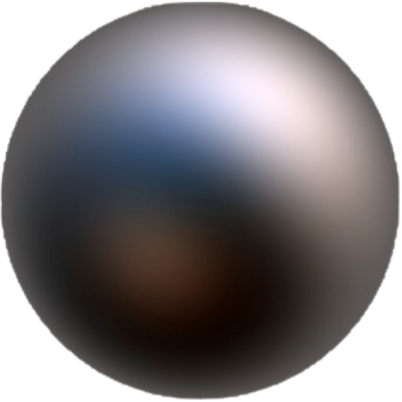
\includegraphics[width=32bp]{\lumigaussassets/folder_for_kacper/rotating/env1.png}};
        \node[anchor=north west] at (scene2-1-1.north west) {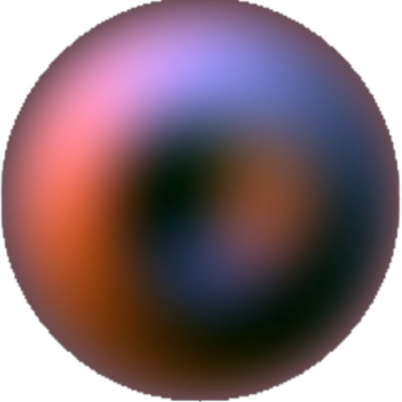
\includegraphics[width=32bp]{\lumigaussassets/folder_for_kacper/rotating/env2.png}};
      \end{tikzpicture}
    }
  }
}

\begin{figure}[!t]
  \centering
  % \includegraphics[width=\linewidth]{images/wild2d-rotate_light_more_items.pdf}
  \rotatingfigure
  \caption{\textbf{Environment map rotation --}
    The top row shows the illumination entering the scene.
    The second and third rows display the shadowed and unshadowed renderings,
    respectively.
    The last row represents the approximate predicted shadows.
    % Note that shadows appear even in brightly illuminated areas, indicating
    % that this is not a result of a dark environment map. 
    Please zoom in for details.
  }
  \label{fig:lumigauss-rotate_light}
\end{figure}
    % \subsection{Relightning capabilities}
    As our backbone, 2DGS~\cite{huang20242d} incorporates priors to produce
    sharp edges and smooth surfaces, our model inherently performs better as
    expressed by SSIM.
    Please also see the zoom-ins
    in~\cref{fig:lumigauss-qual_albedo_norm_relight}.
    Those shape reconstruction qualities allow us to relight the scene with
    high fidelity.
    We demonstrate that in~\cref{fig:lumigauss-rotate_light} where one can see
    that our method effectively relights landmarks under various lighting
    conditions.
    We finally visualize the rendered shadows produced thanks to our proposed
    physical constraints at training time.
    Since \lumigauss does not predict shadows explicitly, we visualize them as grayscaled difference of output irradiances between the \textit{unshadowed} (\cref{eq:lumigauss-unshadowed-radiance}) and \textit{shadowed} (\cref{eq:lumigauss-shadowed-radiance}) to approximate shadow effects:
    \begin{equation}
      \max(\mathfrak{g}(\radiance_k \oslash \albedo_k - \shadowedradiance_k \oslash \albedo_k), 0),
    \end{equation}
    where $\oslash$ is an element-wise division and $\mathfrak{g}(\cdot)$ converts from the RGB space to the grayscale space.

    We also display the illumination in~\cref{fig:lumigauss-rotate_light} to
    differentiate between shadows and dark illumination from the environment
    map.
    Additional detailed results on scene reconstruction, relightning and more
    comparisons to other works are included in~\supplementary{}.

  \subsection{Ablations}

    We prioritize enhancing relighting capabilities over accurate appearance
    recreation during the optimization process, contrasting with recent
    Gaussian splatting methods that target novel view synthesis based on
    unconstrained photo
    collections~\cite{xu2024wildgs,dahmani2024swagsplattingwildimages,zhang2024gaussian}.
    Consequently, our ablation study primarily focuses on the degradation of
    relighting capabilities when removing any of the proposed components.
    We compare shadowed and unshadowed modeling and investigate the
    contributions of each loss term.
    We present the results in \cref{tab:lumigauss-results_osr_eval}.
    % We provide additional results in~\supplementary{}.

    Gaussians can optimize to shadowed surfaces and represent shadows as
    normals and albedo colors (effect known as albedo/illumination ambiguity).
    Therefore, gains from separating shadows from lightning are not visible in
    metrics computed on a limited data subset.
    We noticed that adding a shadowed version can help restore proper albedo
    and normal vectors of surfaces that during the training were distorted or
    had low brightness (see \cref{fig:lumigauss-shadowed_fix_normals}).

  \subsection{Performance comparison}
    We compare \lumigauss' efficiency with two NeRF baselines.
    Our method achieves plausible relightning results while being orders of
    magnitudes faster both in terms of training and inference as shown in
    \cref{tab:lumigauss-performance}.
    % %%%%%%%%%%%%%%%%%%%%%%%%%%%%%%%%%%%%%%%%%%%%
  \subsection{Limitations}
    We identify the following limitations of our approach.
    Notably, surface albedo and normals may attempt to simulate shadows in
    scenarios with hard and frequent shadows.
    This can pose challenges for shadow training, especially when shadows are
    visible in several training images, potentially hindering the accurate
    representation of surface normals.
    Incorporating priors for environment light and shadowing could further
    enhance disentanglement and light transport modeling as presented in the
    concurrent NeuSky~\cite{gardner2023neusky}.
    While we assume diffuse albedo, valid for most outdoor cases, shadows can
    appear unnaturally on reflective surfaces such as windows.
    Separate background optimization could enhance the synthesis of scenes
    with extensive sky areas.
    Finally, our shadow modeling baked-in the spherical harmonics
    representations is non trivial to extend to dynamic applications, such as
    autonomous driving.
